\documentclass{sig-alternate}
\usepackage{amsmath,amssymb}
\usepackage{graphicx}
\usepackage{hyperref}
\usepackage{color}
\usepackage{algorithm}
\usepackage[noend]{algorithmic}

\newcommand{\comment}[1]{}
\newcommand{\compiler}{Serjeant}
\newcommand{\todo}[1]{\textcolor{red}{#1}}
\newcommand{\feature}[1]{\textbf{#1.}}
\newcommand{\tuple}[1]{{\langle#1\rangle}}
\newcommand{\bigsum}{bigsum}

\newtheorem{theorem}{Theorem}[section]
\newtheorem{metatheorem}{Metatheorem}[section]
\newtheorem{example}[theorem]{Example}
%\newtheorem{algorithm}[theorem]{Algorithm}
\newtheorem{definition}[theorem]{Definition}
\newtheorem{proposition}[theorem]{Proposition}
\newtheorem{property}[theorem]{Property}
\newtheorem{corollary}[theorem]{Corollary}
\newtheorem{lemma}[theorem]{Lemma}
\newtheorem{remark}[theorem]{Remark}
\newtheorem{conjecture}[theorem]{Conjecture}
\newtheorem{proviso}[theorem]{Proviso}

\graphicspath{{../figures}{./figures}}

\begin{document}
\title{Serjeant: Compiling Databases for High-Performance View Maintenance and Update Stream Processing}
\numberofauthors{2}
\author{
\alignauthor Yanif Ahmad\\
    \affaddr{Computer Science Dept.}\\
    \affaddr{Cornell University}\\
    \email{yanif@cs.cornell.edu}
\alignauthor Christoph Koch\\
    \affaddr{Computer Science Dept.}\\
    \affaddr{Cornell University}\\
    \email{koch@cs.cornell.edu}
}
\maketitle

\begin{abstract}
We present \compiler, a novel SQL query compiler for generating database engines
for high-performance main-memory processing of streaming data. \compiler\
aggressively compiles aggregate queries to C++ code, to perform incremental view
maintenance of continuous queries posed on streaming data. While today's
state-of-the-art view maintenance considers a single delta on each input
relation, \compiler\ uses a recursive compilation technique to successively
simplify queries, exploiting combinations of input deltas to eliminate joins,
and factorize aggregates. \compiler\ automatically determines subparts of
queries to eagerly maintain as map data structures during compilation, and
generates code that both computes query results from maps, and maintains maps
given their interdependencies.  \compiler\ is capable of generating incremental
engines for a wide range of aggregate queries, including nested aggregate
queries with predicates, which to the best of our knowledge has not been
addressed in the literature.  Our work is motivated by applications that require
the highly efficient answering of fixed workloads of aggregation queries, such
as in data stream processing, online data warehouse loading, and in financial
applications. As we show, our techniques are at least one to two orders of
magnitude faster than state-of-the-art database and stream processing engines on
such workloads.
\end{abstract}



In recent years, algorithmic trading systems have come to account for a majority
of volume traded at the major US and European financial markets (for instance,
for 73\% of all US equity trading volume in the first quarter of 2009
\cite{Iati2009}). The success of automated trading systems depends critically on
strategy processing speeds: trading systems that react faster to market events
tend to make money at the cost of slower systems. Unsurprisingly, algorithmic
trading has become a substantial source of business for the IT industry; for
instance, it is the leading vertical among the customer bases for high-speed
switch manufacturers (e.g., Arista \cite{Becht2010}) and data stream processing.




A typical algorithmic trading system is run by mathematicians who develop
trading strategies and by programmers and systems experts who implement these
strategies to perform fast enough, using mainly low-level programming languages
such as C. Developing trading strategies requires a feedback loop of simulation,
back-testing with historical data, and strategy refinement based on the insights
gained. This loop, and the considerable amount of low-level programming that it
causes, is the root of a very costly {\em productivity bottleneck}\/: in fact,
the number of programmers often exceeds the number of strategy designers by
an order of magnitude.


Trading algorithms often perform a considerable amount of data crunching
and statistical processing that could in principle be implemented using SQL
views, coupled with some relatively straightforward control and trading logic.
%
Differently from other areas of finance such as technical analysis,
where stream processing engines
\cite{abadi-vldbj:03,motwani-cidr:03} can be applied,
data processing in trading algorithms using views cannot be performed by DBMS or
data stream processing systems today: the former are not able to (1) {\em update
their views at the required rates}\/ (for popular stocks, hundreds of orders per
second may be executed, even outside burst times) and the latter are not able to
(2) {\em maintain large enough data state}\/ and support suitable query
languages (non-windowed SQL aggregates) on this state.

%
A data management system that could handle these two requirements would yield a
very substantial productivity increase that can be directly monetized -- the
holy grail of algorithmic trading.

Trading algorithms often perform a considerable amount of data crunching that
could in principle be implemented as SQL views, but cannot be achieved by DBMS
or data stream processing systems today: DBMS are not able to (1) {\em update
their views at the required rates}\/ (for popular stocks, hundreds of orders per
second may be executed, even outside burst times) and stream engines are not
able to (2) {\em maintain large enough data state}\/ and support suitable query
languages (non-windowed SQL aggregates) on this state.
A data management system fulfilling these two requirements would yield a very
substantial productivity increase that can be directly monetized -- the holy
grail of algorithmic trading.



To understand the need to maintain and query a large data state, note that
many stock exchanges provide a detailed view of the market microstructure
through complete bid and ask {\em limit order books}. The bid order book is a
table of purchase offers with their prices and volumes, and correspondingly the
ask order book indicates investors' selling orders. Exchanges execute trades by
matching bids and asks by price and favoring earlier timestamps. Investors
continually add, modify or withdraw limit orders, thus one may view order books
as relational tables subject to high update volumes. The availability of order
book data has provided substantial opportunities for automatic algorithmic
trading.





To illustrate this, we describe the Static Order Book Imbalance (SOBI) trading
strategy. SOBI computes a volume-weighted average price (VWAP) over those orders
whose volume makes up a fixed upper $k$-fraction of the total stock volume in
both bid and ask order books. SOBI then compares the two VWAPs and, based on
this, predicts a future price drift (for example a bid VWAP larger than an ask
VWAP indicates demand exceeds supply, and prices may rise). For simplicity, we
present the VWAP for the bids only:



\begin{verbatim}
select avg(b2.price * b2.volume) as bid_vwap
from   bids b2
where  k * (select sum(volume) from bids)
         > (select sum(volume) from bids b1
            where b1.price > b2.price);
\end{verbatim}
\comment{
Focusing on the $k$-fraction of the order book closest to the current price
makes the SOBI strategy less prone to attacks known as {\em axes}\/ (large
tactical orders far from the current price that will thus not be executed but
may confuse competing algorithms).
}


Coming back to our two desiderata, for trading algorithms to be successful, (1)
views such as VWAP need to be maintained and monitored by the algorithms at or
close to the trading rate. However, (2) the views cannot be expressed through
time-, row- or punctuation-based window semantics.




\section{Query Compilation}


\def\algsum{\mathrm{sum}}
\def\algagg{\mathrm{agg}}
\def\algtop{\mathrm{top}}
\def\algtopk{\mathrm{topk}}



This section presents our framework for compiling aggregation queries down to
efficient procedural code for incrementally maintaining views of these queries.
We start with a definition of a clean
core of the query language supported by DBToaster.
This core is a query algebra for defining maps. These maps are closely related to
tables definable using SQL aggregate group-by queries but at the same time are main
memory data structures that are easy to access in applications.
After that, we present the core query compilation technique and prove its correctness.
In the following subsection, we refine this technique to employ join decomposition
techniques or employ database query optimization ideas to reduce the space
consumption of auxiliary maps and to reduce the time cost of maintaining the maps.




\subsection{The Map Algebra}


\def\algsumr{\mbox{sumr}}
\def\algsumf{\mbox{sumf}}
\def\distinct{\mbox{distinct}}
\def\routerjoin{\bowtie\!=}


The syntax of the map algebra can be defined as follows.
Inductively, a map algebra expression is of one of the forms $f_1 + f_2$,
$f_1 - f_2$, $f_1 * f_2$, $f_1 / f_2$, $c$, $x$, and $\algsumf_A(Q)[\vec{x}]$,
where $f_1$ and $f_2$ are map algebra expressions, $c$ are numerical constants,
$x$ is a variable, $\vec{x}$ is a tuple of variables, $Q$ is a relational algebra
expression, and $A$ is a column name of the schema of the relation defined by $Q$.
We call the arity of the variable tuple of a map its {\em dimension}\/.
Relational algebra expressions are built using relation names,
selection $\sigma$, projection $\pi$, relational product $\times$, union $\cup$,
and renaming $\rho$. (Note the absence of the relational difference operation
at this point; we
relax this restriction later.) Selection conditions are comparisons
$f = 0$, $f > 0$, or $f \ge 0$.
Projections may compute additional columns
using map algebra expressions. 
The variables from $\vec{x}$ may be used in
any map algebra expression used in selections or projections of $Q$.

We use a multiset semantics for relations as in SQL; none of the operations
of relational algebra eliminate duplicates.
Apart from that, the semantics of relational algebra expressions $Q$ is standard.
Variables
in $\vec{x}$ are {\em bound}\/ to constants from above; thus, the semantics of an
aggregate map $\algsumf_f(Q)[\vec{x}]$, where $\vec{x}$ is bound to a tuple of
constants $\vec{a}$
(denoted $\algsumf_f(Q)[\vec{a}]$) is a single numerical value $v$ such that, if
$Q[\vec{a}]$ is $Q$ with the variables $\vec{x}$ substituted with the constants
$\vec{a}$ and $\algsumr_A$ is the standard sum aggregate function of SQL,
\[
\algsumr_A(Q[\vec{a}])[] = \{ \tuple{v} \}.
\]


\begin{remark}\em
Thus, while nongrouped aggregation in SQL corresponds to our semantics of aggregate
maps $f[]$ of dimension zero apart from syntax (the result of $f[]$ is a scalar number
while the result of the SQL aggregate is a singleton unary relation),
the semantics of aggregate maps $f[\vec{x}]$ of higher dimension differs from that
of SQL group-by in that $f[\vec{x}]$ is a complete function defined anywhere
(indeed, $\algsumr_B(\sigma_{\vec{A}=\vec{a}}(Q))$ produced $\{\tuple{0}\}$ rather
than no tuple at all when $\sigma_{\vec{A}=\vec{a}}(Q)$ is the empty relation) while
the SQL aggregate-group-by query
$\sigma_{\vec{A}=\vec{a}}$(select $\vec{A}$, sum$(B)$ from $Q$ group by $\vec{A}$)
gives no value on tuples $\vec{a}$ that do not exists in $\pi_{\vec{A}}(Q)$.

Thus, for our purposes, SQL group-by aggregates do not generalized non-grouped
SQL aggregates. We avoid this in our map algebra -- this allows for a clean
compositional compilation framework, and to focussing on the essential challenges
below. Still, the map algebra supports a wide range of practical queries, and we will
generalize it later to support even more once we have laid the necessary foundations.
\end{remark}


\begin{example}\em
The VWAP query from the introduction was, in algebra notation with $\distinct$
denoting
tuple elimination and $\routerjoin$ denoting right outer join,
\begin{multline*}
\algsumr_{P_2 * V_2}(\algsumr_{V_0 \rightarrow S_0}(\rho_{P_0, V_0}(B))
\; \bowtie_{k * S_0 > S_1} \\
\algsumr_{V_1 \rightarrow S_1 \;\mathrm{grpby}\; P_2}(
\rho_{P_1, V_1}(B) \; \routerjoin_{P_1 > P_2} \\
\distinct(\pi_{P_2}(\rho_{P_2, V_2'}(B)))) \bowtie \rho_{P_2, V_2}(B)).
\end{multline*}
This translates via 
\begin{multline*}
\algsumf_{P_2 * V_2}(
\pi_{m_0[]  \rightarrow S_0}(\{\tuple{}\})
\; \bowtie_{k * S_0 > S_1} \\
\pi_{P_2, m_1[P_2] \rightarrow S_1}
(\distinct(\pi_{P_2}(\rho_{P_2, V_2'}(B)))) \bowtie \rho_{P_2, V_2}(B))[]
\end{multline*}
%
where the maps $m_0$ and $m_1$ are
\begin{eqnarray*}
m_0[] &:=&
\algsumf_{V_0}(\rho_{P_0, V_0}(B))[]
\\
m_1[p_2] &:=&
\algsumf_{V_1}(\sigma_{P_1 > p_2}(\rho_{P_1, V_1}(B)))[p_2]
\end{eqnarray*}
to our map algebra:
\begin{multline*}
\algsumf_{P_2 * V_2}(
\sigma_{k * S_0 > S_1}( \\
\pi_{m_0[]  \rightarrow S_0, P_2, m_1[P_2] \rightarrow S_1}
(\distinct(\pi_{P_2}(\rho_{P_2, V_2'}(B))))) \bowtie \rho_{P_2, V_2}(B))[]
\end{multline*}
The query can be simplified using standard relational algebra equivalences
further to
\[
q[] = \algsumf_{P_2 * V_2}(
\sigma_{k * S_0 > S_1}(
\pi_{m_0[]  \rightarrow S_0, m_1[P_2] \rightarrow S_1, P_2, V_2}
(\rho_{P_2, V_2}(B))))[]
\]
and to
\begin{equation}
q[] = \algsumf_{P_2 * V_2}(
\sigma_{m[P_2] > 0}(\rho_{P_2, V_2}(B)))[]
\end{equation}
where
\[
m[p_2] = k * m_0[] - m_1[P_2].
\]
\punto
\end{example}



\subsection{Compiling Queries: Foundations}


The goal of this section is to provide an algorithm for compiling map algebra
expressions into efficient C code that incrementally maintains the
maps they define.
To be precise, we aim for the following notion of incremental maintenance.


\begin{definition}[YMCA maintenance scheme]\em
An incremental map maintenance algorithm has the YMCA
(Yanif Must Certainly Approve of)
property if on an insert or delete of a tuple, the delta on $q[\vec{a}]$, for
any $\vec{a}$, can be expressed as a fixed sum
$q_1[\vec{a}] + \dots + q_k[\vec{a}]$ such that each map $q_i[\cdot]$ has the YMCA
property and $q_i \prec q$.
\end{definition}


Here, $\prec$ denotes the following general-to-specific ordering on map expressions.


\begin{definition}\em
A singleton relation is a relation with one tuple, e.g.\ $\{\vec{a}\}$.
A map $q$ is called (strictly) {\em more specific than}\/ a map $q'$,
denoted $q \prec q'$, if $q$ can be obtained from $q'$ by replacing
one or more relation names occurring in $q$ by fixed singleton relations.
\end{definition}


Obviously, a YMCA compilation scheme yields effective incremental view maintenance:
The delta to any map can be computed by a fixed sum of simpler maps,
the deltas of which again can be computed by fixed sums of even simpler maps,
and this recursively until we reach maps in which all relations are constant and
the maps can be reformulated as a simple arithmetic expressions over their
arguments.



\begin{theorem}
There is a YMCA compilation scheme for map algebra.
\end{theorem}


Proof.
Let $q[\vec{x}]$ be of the form
$
\algsumf_f(Q)[\vec{x}]
$
where $Q$ is relational algebra parameterized by $\vec{x}$ and let $R$ be
a relation name occurring in $Q$ (in the relational algebra expression
rather than just in a nested map algebra expression).
Assume that there are $r$ occurrences of $R$ in $Q$. Then
the updated version of $q[\vec{x}]$ can be expressed by the sum of the $2^r$
maps obtainable by, for each occurrence of $R$ in $Q$, either replacing it
by $\{ \vec{x} \}$ or leaving it unchanged.

This follows immediately from the fact that the new version of $R$ on insertion of
tuple $\vec{x}$ is $R \cup \{ \vec{x} \}$ and, $\cup$ commutes with
the operations of positive relational algebra and thus can be pushed to the top
level of $Q$, and
\[
\algsumf_f(Q_1 \cup Q_2)[\vec{x}] =
\algsumf_f(Q_1)[\vec{x}] + \algsumf_f(Q_2)[\vec{x}].
\]
By pushing the unions obtained by rewriting $R$ to $R \cup \{\vec{x}\}$ to the
top level of $Q$ everywhere and then splitting the map into a sum of maps, we obtain
one map expression that is precisely $q[\cdot]$ (i.e., corresponds to the old
value of $q$).

The one additional case is relational algebra expressions of the form
\[
\algsumf_f(\sigma_{m[\vec{x}] + \Delta m[\vec{x}] > 0}(Q))[\cdot]
\]
which can be rephrased as
\begin{multline*}
\algsumf_f(\sigma_{m[\vec{x}] > 0}(Q))[\vec{x}]
\\
+ \;
\big( \mbox{if ($(m[\vec{x}] > 0) \neq (m[\vec{x}] + \Delta m[\vec{x}] > 0))$ then}
\\
      \mbox{$\mbox{sgn}(m[\vec{x}] + \Delta m[\vec{x}]) *
      \algsumf_f(Q)[\vec{x}]$ else 0} \big)
\end{multline*}
\punto



\begin{todo}
Make a clean induction proof.

Give an algorithm separately from the proof.
\end{todo}



\begin{example}\em
Let us now compute the trigger
\[
\mbox{on insert into B values ($p, v$)}
\]
for the VWAP query $q[]$.
If we replace $B$ by $B \cup \{\tuple{p, v}\}$ everywhere
%
%and use the equivalences
%$\pi_{\vec{A}}(R \cup S) = \pi_{\vec{A}}(R) \cup \pi_{\vec{A}}(S)$ and
%$\algsumf_f(R \cup S)[\vec{x}] =
%\algsumf_f(R)[\vec{x}] + \algsumf_f(S)[\vec{x}]$,
we obtain that $q[]$ should be incremented by
%
\begin{eqnarray*}
\Delta q[] &=&
\sum_{p_2}
\big( \mbox{if ($(m[p_2] > 0) \neq (m[p_2] + \Delta m[p_2] > 0))$ then}
\\
&& ~~~
      \mbox{$\mbox{sgn}(m[p_2] + \Delta m[p_2]) *
      \underbrace{\algsumf_{P_2 * V_2}(\sigma_{P_2=p_2}(\rho_{P_2,V_2}(B)))[p_2]}_{s[p_2]}$ else 0} \big)
\\
%&+& \algsumf_{p_2 * v_2}(\sigma_{m[p_2] + \Delta m[p_2] > 0}(
%\rho_{P_2, V_2}(\{\tuple{p_2,v_2}\})))[]
%\\
&+&
\big( \mbox{if $(m[p] + \Delta m[p] > 0)$ then $p * v$ else $0$} \big)
\end{eqnarray*}

The increments for $m[P_2]$ and $s[P_2]$
on insertion of tuple $\tuple{p,v}$ into $B$ are
analogously
\begin{eqnarray*}
\Delta m[p_2] &:=&
k * \algsumf_{V_0}(\rho_{P_0, V_0}(\{\tuple{p, v}\}))[] -
\algsumf_{V_1}(\sigma_{P_1 > p_2}(\rho_{P_1, V_1}\{\tuple{p, v}\})))[p_2]
\\
&=& k * v - (\mbox{if $(p > p_2)$ then $v$ else $0$)}
\\
&& (\mbox{for each $p_2$})
\\[1.5ex]
\Delta s[p_2] &:=& \mbox{if $(p = p_2)$ then v else 0}.
\end{eqnarray*}

Thus we generate the following code:
\begin{verbatim}
on insert into B values (p, v)
{
  if(! dom_m.member(p)) { dom_m.add(p); m[p] = 0; }

  delta q = (m[p] > 0) ? (p * v) : 0;

  foreach p_2 in dom_m do
  {
     delta m[p_2] = k * v - ((p > p_2) ? v : 0);
     delta s[p_2] = (p = p_2) ? v : 0;
     delta q += ((m[p_2] > 0) != (m[p_2] + delta m[p_2] > 0)) ?
        sgn(m[p_2] + delta m[p_2]) * (s[p_2] + delta s[p_2]) : 0;
  }

  increment the maps by their deltas;
}
\end{verbatim}


It makes sense to avoid naive looping over all values $p_2$ by maintaining
$m_1[p_2]$ as a range data structure (to be described).
\punto
\end{example}







%%%%%%%%%%%%%%%%%%%%%%%%%%%%%%%%%%%



\section{Old Stuff}






\begin{figure*}
\begin{eqnarray}
\rho_{\vec{A}\vec{B}}(R) \bowtie \rho_{\vec{A}\vec{C}}(\{ \tuple{\vec{a}\vec{c}} \})
&\vdash&
\sigma_{\vec{A}=\vec{a}}(\rho_{\vec{A}\vec{B}}(R)) \times \rho_{\vec{C}}(\{ \vec{c} \})
\label{r1}
\\
\pi_{\vec{A}}(\rho_{\vec{A}}(R) \times \rho_{\vec{B}}(\{ \vec{b} \}))
&\vdash&
\rho_{\vec{A}}(R)
\label{r2}
\\
\rho_{\vec{A}}(\{\vec{a}\}) \times \rho_{\vec{B}}(R)
&\vdash&
\sigma_{\vec{A}=\vec{a}}(\rho_{\vec{A}}(\{\vec{a}\}) \times \rho_{\vec{B}}(R))
\label{r3}
\\
\algagg_{f(\vec{A},\vec{B})}(\sigma_{\vec{A}=\vec{a}}(R))
&\vdash&
\algagg_{f(\vec{a},\vec{B})}(\pi_{\vec{B}}(R))
\label{r4}
\\
\algagg_{f(\vec{A})}(\rho_{\vec{A}}(R) \times \rho_{\vec{B}}(\{\vec{b}\}))
&\vdash&
\algagg_{f(\vec{A})}(\rho_{\vec{A}}(R))
\label{r5}
\\
\algsum_{f(\vec{A}) * g(\vec{B})}(\rho_{\vec{A}}(R) \times \rho_{\vec{B}}(S))
&\vdash&
\algsum_{f(\vec{A})}(\rho_{\vec{A}}(R)) *
\algsum_{g(\vec{B})}(\rho_{\vec{B}}(S))
\label{r6}
\\
\algsum_{a *
f(\cdot)}(R) &\vdash& a * \algsum_{f(\cdot)}(R)
\label{r7}
\\
\algsum_{f(\cdot) + g(\cdot)}(R)
&\vdash&
\algsum_{f(\cdot)}(R) + \algsum_{g(\cdot)}(R)
\label{r8}
\\
\max_{a + f(\cdot)}(R)
&\vdash&
a + \max_{f(\cdot)}(R)
\label{r9}
\\
\max_{f(\vec{A}) + g(\vec{B})}(\rho_{\vec{A}}(R) \times \rho_{\vec{B}}(S))
&\vdash&
\max_{f(\vec{A})}(\rho_{\vec{A}}(R)) +
\max_{g(\vec{B})}(\rho_{\vec{B}}(S))
\label{r10}
\\
\max_{a * f(\vec{B})}(\rho_{\vec{B}}(R))
&\vdash&
\left\{
\begin{array}{lll}
a * \min_{f(\vec{B})}(\rho_{\vec{B}}(R)) & \dots & a < 0 \\
a * \max_{f(\vec{B})}(\rho_{\vec{B}}(R)) & \dots & a \geq 0
\end{array}
\right.
\label{r11}
\\
\max_{f(\vec{A}) * g(\vec{B})}(\rho_{\vec{A}}(R) \times \rho_{\vec{B}}(S))
&\vdash&
\max\Big\{
\max_{f(\vec{A})}(\sigma_{f(\vec{A}) \ge 0}(\rho_{\vec{A}}(R))) *
\max_{g(\vec{B})}(\rho_{\vec{B}}(S)),
\nonumber\\
&& \quad\quad\;\;\,
\max_{f(\vec{A})}(\underbrace{\sigma_{f(\vec{A}) < 0}}_{\mathrm{optional}}(\rho_{\vec{A}}(R))) *
\max_{g(\vec{B})}(\sigma_{f(\vec{B}) \ge 0}(\rho_{\vec{B}}(S))),
\nonumber\\
&& \quad\quad\;\;\,
\min_{f(\vec{A})}(\sigma_{f(\vec{A}) < 0}(\rho_{\vec{A}}(R))) *
\min_{g(\vec{B})}(\sigma_{f(\vec{B}) < 0}(\rho_{\vec{B}}(S)))
\Big\}
\label{r12}
\\
\max_a(R)
&\vdash&
\left\{
\begin{array}{lll}
a       & \dots & \algsum_1(R) > 0 \\
-\infty & \dots & \algsum_1(R) = 0 \\
\end{array}
\right.
\label{r13}
\end{eqnarray}

\caption{Rewrite rules. agg can be either sum, max, or min.
count is sum$_1$.}
\label{fig:rules}
\end{figure*}



\begin{figure*}
\begin{eqnarray}
\algsum_{f(\cdot)}(R - S)
& \vdash &
\algsum_{f(\cdot)}(R) -
\algsum_{f(\cdot)}(S) \quad \dots \quad S \subseteq R
\label{r20}
\\
\max_{f(\cdot)}(R - S)
& \vdash &
\left\{\begin{array}{lll}
\max_{f(\cdot)}(R) & \dots & (S \cap R = \emptyset) \vee \\
& &  (\max_{f(\cdot)}(R) \neq
\max_{f(\cdot)}(S \cap R)) \\
\max_{f(\cdot)}(R
- S) & \dots &  \max_{f(\cdot)}(R) = \max_{f(\cdot)}(S \cap R) \\
\end{array}\right.
\label{r21}
\\
\rho_{\vec{A}\vec{B}}(R) \bowtie \rho_{\vec{A}\vec{C}}(S)
& \vdash &
\bigcup_{\vec{a}}
\sigma_{\vec{A}=\vec{a}}(\rho_{\vec{A}\vec{B}}(R))
\times \sigma_{\vec{A}=\vec{a}}(\rho_{\vec{A}\vec{C}}(S))
\label{r23}
\\
\max_{f(\vec{A},\vec{B},\vec{C})} \Big\{
\bigcup_{\vec{a}}
\sigma_{\vec{A}=\vec{a}}(\rho_{\vec{A}\vec{B}}(R)) \times
\sigma_{\vec{A}=\vec{a}}(\rho_{\vec{A}\vec{C}}(S)) \Big\}
& \vdash &
\max_{f(\vec{A},\vec{B},\vec{C})}\Big\{
\bigcup_{\vec{a}} \max_{f(\vec{a},\vec{B},\vec{C})}
(\sigma_{\vec{A}=\vec{a}}(\rho_{\vec{A}\vec{B}}(R)) \times
\sigma_{\vec{A}=\vec{a}}(\rho_{\vec{A}\vec{C}}(S))) 
\Big\}
\label{r24}
\end{eqnarray}
\caption{Rewrite rules for handling deletions. Note that deletion rewrites use
both this rule set and the rewrite rules above for insertions.}
\label{fig:deleterules}
\end{figure*}





\nop{
\begin{figure*}
\begin{eqnarray}
\mathop{\algtopk}_{a+f(\cdot)}(R)
&\vdash&
\pi_{a+f(\cdot)}(\{\tuple{a}\} \times
\mathop{\algtopk}_{f(\cdot)}(R))
\label{r14}
\\
\mathop{\algtopk}_{f(\vec{A}) + g(\vec{B})}(\rho_{\vec{A}}(R) \times
\rho_{\vec{B}}(S))
&\vdash&
\mathop{\algtopk}(\pi_{f(\vec{A}) + g(\vec{B})}(
\mathop{\algtopk}_{f(\vec{A})}(\rho_{\vec{A}}(R))
\times \mathop{\algtopk}_{g(\vec{B})}(\rho_{\vec{B}}(S))))
\label{r15}
\\
\mathop{\algtopk}_{a * f(\vec{B})}(\rho_{\vec{B}}(R))
&\vdash&
\left\{
\begin{array}{lll}
\pi_{-a*-f(\vec{B})}( \{\tuple{a}\} \times
\mathop{\algtopk}_{-f(\vec{B})}(\rho_{\vec{B}}(R))) &
\dots & a < 0 \\
\pi_{a*f(\vec{B})}( \{\tuple{a}\} \times 
\mathop{\algtopk}_{f(\vec{B})}(\rho_{\vec{B}}(R))) & \dots & a \geq 0
\end{array}
\right.
\label{r16}
\\
\mathop{\algtopk}_{f(\vec{A}) * g(\vec{B})}(\rho_{\vec{A}}(R)
\times \rho_{\vec{B}}(S))
&\vdash&
\mathop{\algtopk} \Big\{
\pi_{f(\vec{A}) * g(\vec{B})}(
\mathop{\algtopk}_{f(\vec{A})}(
\sigma_{f(\vec{A}) > 0}(\rho_{\vec{A}}(R))) \times
\mathop{\algtopk}_{g(\vec{B})}(\rho_{\vec{B}}(S))),
\nonumber\\
& &
\pi_{f(\vec{A}) * g(\vec{B})}(
\mathop{\algtopk}_{f(\vec{A})}
(\rho_{\vec{A}}(R)) \times
\mathop{\algtopk}_{g(\vec{B})}
(\sigma_{g(\vec{B}) > 0}(\rho_{\vec{B}}(S))))
\nonumber\\
& &
\pi_{-f(\vec{A}) * -g(\vec{B})}(
\mathop{\algtopk}_{-f(\vec{A})}
(\sigma_{f(\vec{A}) < 0}(\rho_{\vec{A}}(R))) \times
\mathop{\algtopk}_{-g(\vec{B})}
(\sigma_{g(\vec{B}) < 0}(\rho_{\vec{B}}(S))))
\Big\}
\label{r17}
\\
\mathop{\algtopk}_{a}(R)
&\vdash&
\left\{\begin{array}{lll}
\{\underbrace{\tuple{a}, \dots, \tuple{a}}_{k \; \mathrm{times}}\} & \dots & \algsum_{1}(R) > k\\
\{\underbrace{\tuple{a}, \dots, \tuple{a}}_{\algsum_{1}(R) \; \mathrm{times}}\}
\cup \{\tuple{-\infty}\}^{k-\algsum_{1}(R)}
& \dots & \algsum_{1}(R) < k
\end{array}\right.
\label{r18}
\\
\mathop{\algtopk}_{f(\cdot)}(\rho_{\vec{A}}(R) - \rho_{\vec{B}}(S))
& \vdash &
\left\{\begin{array}{lll}
\algtopk_{f(\cdot)}(R) &
\dots & (S \cap R = \emptyset) \vee\\
& & (\algtopk_{f(\cdot)}(R) \cap 
\algtopk_{f(\cdot)}(S \cap R) = \emptyset)\\
\algtopk_{f(\cdot)}(R - S)
& \dots &
\algtopk_{f(\cdot)}(R) \cap
\algtopk_{f(\cdot)}(S \cap R) \neq \emptyset
\end{array}\right.
\label{r22}
\end{eqnarray}
\begin{eqnarray}
\mathop{\algtopk}_{f(\vec{A},\vec{B},\vec{C})} \Big\{
\bigcup_{\vec{a}}
\sigma_{\vec{A}=\vec{a}}(\rho_{\vec{A}\vec{B}}(R)) \times
\sigma_{\vec{A}=\vec{a}}(\rho_{\vec{A}\vec{C}}(S)) \Big\}
& \vdash &
\mathop{\algtopk}_{f(\vec{A},\vec{B},\vec{C})}\Big\{
\bigcup_{\vec{a}} \mathop{\algtopk}_{f(\vec{a},\vec{B},\vec{C})}
(\sigma_{\vec{A}=\vec{a}}(\rho_{\vec{A}\vec{B}}(R)) \times
\sigma_{\vec{A}=\vec{a}}(\rho_{\vec{A}\vec{C}}(S))) 
\Big\}
\label{r25}
\end{eqnarray}
\caption{Rewrite rules for top-k.}
\end{figure*}
} % end nop







In this section, an expression of the form
\[
\algagg_f(\sigma_{\vec{A}=\vec{a}}(Q))[\vec{a}]
\]
is a map for an aggregate-group by query
\[
\mbox{select $\vec{A}$, agg($f$)
from $Q$
group by $\vec{A}$}.
\]
Given a group $\vec{a}$, the map returns
the aggregate value
$\algagg_f(\sigma_{\vec{A}=\vec{a}}(Q))$ for it.
An aggregate $\algagg$ (either sum, max, or min) returns exactly
one value -- the aggregate value.

The main rewrite step is the following.
We exploit the fact that for our aggregate functions $\algagg$,
\begin{multline*}
\algagg_f(\sigma_{\vec{A}=\vec{a}}(Q \cup \Delta Q))[\vec{a}]
= \\
\algagg(\algagg_f(\sigma_{\vec{A}=\vec{a}}(Q))[\vec{a}],
\algagg_f(\sigma_{\vec{A}=\vec{a}}(\Delta Q))[\vec{a}]).
\end{multline*}


Consider an aggregate-group by query
\[
\algagg_{f(\vec{a}, \vec{B}, \vec{C}, \vec{D})}
(\sigma_{\vec{A}=\vec{a}}(R_1 \bowtie \dots \bowtie R_k))[\vec{a}]
\]
where the schema of $R_1 \bowtie \dots \bowtie R_{k-1}$ is
$\vec{A}\vec{B}\vec{C}$ and the schema of
$R_k$ is $\vec{C}\vec{D}$.

W.l.o.g., we consider the case of an insertion of tuple
$\tuple{\vec{c},\vec{d}}$ into relation $R_k$.

We rewrite
$
\algagg_f(\sigma_{\vec{A}=\vec{a}}(\Delta Q))[\vec{a}]
$, that is,
\[
\algagg_{f(\vec{a}, \vec{B}, \vec{C}, \vec{D})}
(\sigma_{\vec{A}=\vec{a}}(R_1 \bowtie \dots \bowtie R_{k-1} \bowtie \{\tuple{\vec{c}\vec{d}}\}))[\vec{a}]
\]
to
\begin{equation}
\algagg_{f(\vec{a}, \vec{B}, \vec{c}, \vec{d})}
(\sigma_{\vec{A}\vec{C}=\vec{a}\vec{c}}(R_1 \bowtie \dots \bowtie R_{k-1}))[\vec{a}\vec{c}\vec{d}].
\label{eq:1}
\end{equation}

Figure~\ref{fig:rules} provides a set of rewrite rules, of which rules
\ref{r1}, \ref{r2}, \ref{r3}, and \ref{r4} are sufficient to  perform this
rewriting.

Since we would like the maps that have to be maintained to be as simple as
possible, we will try to express Equation~\ref{eq:1} in terms of 
aggregates
\begin{equation}
\algagg_{f'(\vec{a}, \vec{B}, \vec{c})}
(\sigma_{\vec{A}\vec{C}=\vec{a}\vec{c}}(R_1 \bowtie \dots \bowtie R_{k-1}))[\vec{a}\vec{c}]
\label{eq:2}
\end{equation}
which do not use $\vec{d}$.

In most cases
this is possible using the rewrite rules of Figure~\ref{fig:rules}.
Assuming that $f$ is an arithmetic expression built using addition and multiplication (and constants which may be negative), we can turn $f$ into an equivalent
expression that is a sum of products (by exploiting distributivity).

Let the aggregate be sum. In that case the rewriting of Equation~\ref{eq:1}
so as to eliminate the constants $\vec{d}$
is always possible using the rules \ref{r7} and \ref{r8}.
In the case of max, the rewriting is usually possible. The simplest case
where it is not is $f = B_1 * d + B_2$.


\begin{proposition}
To do: Formalize this fact.
\end{proposition}


Note that our rewriting has removed relation $R_k$ from the query to be
incrementally maintained. Inductively, we can solve the incremental maintenance
problem by just maintaining the maps constructed using this rewriting.


\begin{example}\em
Given schema $R(A,B)$, $S(B,C)$, $T(C,D)$.
We incrementally maintain the aggregate query
\[
s := \algsum_{A*D}(R \bowtie S \bowtie T).
\]
\begin{itemize}
\item
Insert R(a,b):
\begin{eqnarray*}
\Delta s &=& \algsum_{A*D}(\{\tuple{a,b}\} \bowtie S \bowtie T)
\\ &\stackrel{\ref{r1}}{=}&
\algsum_{A*D}(\{a\} \times \sigma_{B=b}(S) \bowtie T)
\\ &\stackrel{\ref{r3},\ref{r4},\ref{r2}}{=}&
\algsum_{a*D}(\sigma_{B=b}(S) \bowtie T)
\\ &\stackrel{\ref{r7}}{=}&
a * \underbrace{\algsum_{D}(\sigma_{B=b}(S) \bowtie T)}_{s_D[b]}
\end{eqnarray*}

\item
Insert S(b,c):
\begin{eqnarray*}
\Delta s &=& \algsum_{A*D}(R \bowtie \{\tuple{b,c}\} \bowtie T)
\\ &\stackrel{\ref{r1}*}{=}&
\algsum_{A*D}(\sigma_{B=b}(R) \times \sigma_{C=c}(T))
\\ &\stackrel{\ref{r6}}{=}&
\underbrace{\algsum_{A}(\sigma_{B=b}(R))}_{s_A[b]} *
\underbrace{\algsum_{D}(\sigma_{C=c}(T))}_{s_D[c]}
\end{eqnarray*}

\item
Insert T(c,d): (analogous to insertion of R(a,b))
\begin{eqnarray*}
\Delta s &=& \algsum_{A*D}(R \bowtie S \bowtie \{\tuple{c,d}\})
\\ &=&
\underbrace{\algsum_{A}(R \bowtie \sigma_{C=c}(S))}_{s_A[c]} * d
\end{eqnarray*}
\end{itemize}

We incrementally maintain $s_D[b]$, $s_A[b]$, $s_D[c]$, and
$s_A[c]$ as well.

\begin{itemize}
\item
Insert R(a,b):
\begin{eqnarray*}
\Delta s_A[b] &=& \algsum_{A}(\{\tuple{a,b}\}) = a
\\
\mbox{foreach $c$: }
\Delta s_A[c] &=& \algsum_{A}(\{\tuple{a,b}\} \bowtie \sigma_{C=c}(S))
\\ &\stackrel{\ref{r1},\ref{r3},\ref{r4},\ref{r2}}{=}&
\algsum_{a}(\sigma_{BC=bc}(S))
\\ &\stackrel{\ref{r7}}{=}&
a * \underbrace{\algsum_{1}(\sigma_{BC=bc}(S))}_{s_1[b,c]}
\end{eqnarray*}

(Analogously insert T(c,d) for maintaining $s_{D}[b], s_{D}[c]$.)

\item
Insert S(b,c):
\begin{eqnarray*}
\Delta s_A[c] &=&
\algsum_{A}(R \bowtie \{\tuple{b,c}\})
\\ &\stackrel{\ref{r1}}{=}&
\algsum_{A}(\sigma_{B=b}(R) \times \{c\})
\\ &\stackrel{\ref{r5},\ref{r2}}{=}&
\algsum_{A}(\sigma_{B=b}(R))
\;=:\; s_A[b]
\\
\Delta s_D[b] &=&
\algsum_{D}(\{\tuple{b,c}\} \bowtie T)
\\ &\stackrel{\ref{r1}}{=}&
\algsum_{D}(\{b\} \times \sigma_{C=c}(T))
\\ &\stackrel{\ref{r5},\ref{r2}}{=}&
\algsum_{D}(\sigma_{C=c}(T))
\;=:\; s_D[c]
\end{eqnarray*}
\end{itemize}

Finally, we want to incrementally maintain $s_1[b,c]$:
\begin{itemize}
\item
Insert S(b,c):
\[
\Delta s_1[b,c] =
\algsum_{1}(\{\tuple{b,c}\}) = 1
\]
\end{itemize}

Thus the code is:
\begin{verbatim}
on insert into R values (a,b)
{
   s += a * s_D[b];
   s_A[b] += a;
   foreach c (in Cs[b]) do
      s_A[c] += a * s_1[b,c];
}

on insert into S values (b,c)
{
   s += s_A[b] * s_D[c];
   s_A[c] += s_A[b];
   s_D[b] += s_D[c];
   s_1[b,c] += 1;
}

on insert into T values (c,d)
{
   s += s_A[c] * d;
   s_D[c] += d;
   foreach b (in Bs[c]) do
      s_D[b] += s_1[b,c] * d;
}
\end{verbatim}
\punto

We can also consider deletions to base relations:

\begin{itemize}
\item
Delete R(a,b):
\begin{eqnarray*}
\algsum &=& \algsum_{A*D}((R-\{\tuple{a,b}\}) \bowtie S \bowtie T)\\
&=& \algsum_{A*D}((R \bowtie S \bowtie T) -
(\{\tuple{a,b}\} \bowtie S \bowtie T))\\
&=& \algsum_{A*D}(R \bowtie S \bowtie T) -\\
& & \algsum_{A*D}(\{\tuple{a,b}\} \bowtie S \bowtie T))\\
&=& \algsum' - \algsum_{A*D}(\{\tuple{a,b}\} \bowtie S \bowtie T))\\
%\because
\Delta s &=&  - \algsum_{A*D}(\{\tuple{a,b}\} \bowtie S \bowtie T))\\
&=& -a*\algsum_{D}(\sigma_{B=b}(S) \bowtie T)
\end{eqnarray*} 
\end{itemize}

(Similarly for Delete S(b,c) and Delete T(c,d)).

Just as in the case for Inserts, we must also maintain an additional data
structures needed by each delta handler, for example $s_{A}[c], s_{A}[b]$ needed
to dealing with deletions to relations S and C. Note that given subtraction is an
inverse operation for addition (hence $\algsum$) and is anticommutative with the
previous result as seen above, the maintenance we perform is
structurally identical to the case for inserts. 

\begin{itemize}
\item
Delete R(a,b):
\begin{eqnarray*}
\Delta s_{A}[b] &=& - \algsum_{A}(\{\tuple{a,b}\}) = -a\\
\Delta s_{A}[c] &=& -a * \algsum_{1}(\sigma_{BC=bc}(S))
\end{eqnarray*}
\end{itemize}
\end{example}


\begin{example}\em
Consider the same query as above where sum is replaced by max,
\[
m := \max_{A*D}(R \bowtie S \bowtie T).
\]

On insert into R values $(a,b)$: $m := \max(m, m')$ where
\begin{eqnarray*}
m' &=&
\max_{A*D}(\{\tuple{a,b}\} \bowtie S \bowtie T)
\\
&\stackrel{\ref{r1},\ref{r3},\ref{r4},\ref{r2}}{=}&
\max_{a*D}(\sigma_{B=b}(S) \bowtie T)
\\
&\stackrel{\ref{r10}}{=}&
\left\{
\begin{array}{lll}
a * \min_{D}(\sigma_{B=b}(S) \bowtie T) & \dots & a < 0 \\
a * \max_{D}(\sigma_{B=b}(S) \bowtie T) & \dots & a \ge 0
\end{array}
\right.
\end{eqnarray*}

For the incremental maintenance of $S$ and $T$, we have to maintain
$\min_A[b] = \min_A(\sigma_{B=b}(R))$,
$\max_A[b] = \max_A(\sigma_{B=b}(R))$,
$\min_A[c] = \min_A(R \bowtie \sigma_{C=c}(S))$ and
$\max_A[c] = \max_A(R \bowtie \sigma_{C=c}(S))$.
For instance,
$\max_A[c] := \max(\max_A[c], \max_A'[c])$
where
\begin{eqnarray*}
\max_A[c] &=&
\max(\max_A[c], \max_A(\{\tuple{a,b}\} \bowtie \sigma_{C=c}(S)))
\\
&\stackrel{\ref{r1},\ref{r3},\ref{r4},\ref{r2}}{=}&
\max(\max_A[c], \max_a(\sigma_{BC=bc}(S)))
\\
&\stackrel{\ref{r12}}{=}&
\left\{
\begin{array}{lll}
\max(\max_A[c], a) & \dots & s_1[b,c] > 0 \\
\max_A[c]          & \dots & s_1[b,c] = 0
\end{array}
\right.
\end{eqnarray*}
where we incrementally maintain
$s_1[b,c] = \algsum_1(\sigma_{BC=bc}(S))$.

Thus the code for maintaining the datastructures on an insert of $R(a,b)$ is
\begin{verbatim}
m = max(m, ((a<0) ? min_D[b] : max_D[b]));
max_A[b] = max(max_A[b], a);
min_A[b] = min(min_A[b], a);
if (s_1[b,c] > 0)
{
   max_A[c] =  max(max_A[c], a);
   min_A[c] =  min(min_A[c], a);
}
\end{verbatim}
\punto
\end{example}

\newcommand{\compile}{\ensuremath{\mbox{\sc Compile}}}
\newcommand{\generate}{\ensuremath{\mbox{\sc Generate}}}
\newcommand{\rewrite}{\ensuremath{\mbox{\sc Rewrite}}}
\newcommand{\substitute}{\ensuremath{\mbox{\sc Substitute}}}
\newcommand{\match}{\ensuremath{\mbox{\sc Match}}}


\def\RETURN{\STATE}


\begin{algorithm}
\caption{$\compile(Q)$}
\label{alg:compile}
\begin{codebox}
\zi \Comment{Inputs: a query $Q$}
\zi \Comment{Outputs: a toasted database $\lambda_{DB}$}
\zi \Comment{Definitions: }
\zi \>$\mathcal{B}$: input tables used by $Q$.
\zi \>$(Q)[]$: initial map (yields query result).
\end{codebox}
\begin{algorithmic}[1]
\STATE $Targets \leftarrow \{\tuple{(Q)[],\mathcal{B}}\}$
\STATE $Kernels \leftarrow \{\}$
\STATE $Maps \leftarrow \{\}$
\WHILE{ $|T| > 0$ }
	\STATE $\tuple{M,\mathcal{R}} \leftarrow next(T)$
	\IF {$|R| = 1$}
		\STATE $Kernel[R] \cup \generate(M,R)$
	\ELSE
		\FOR{$R \in \mathcal{R}$}
			\STATE $\tuple{\{M'\}, \lambda_R} \leftarrow \rewrite(M,R)$
			\STATE $Kernel[R] \leftarrow Kernel[R] \cup \lambda_R$
			\STATE $Targets \leftarrow Targets \cup \{\tuple{M',\mathcal{R}-R}\}$
		\ENDFOR
	\ENDIF
\ENDWHILE
\STATE $\lambda_{DB} \leftarrow \lambda(\Delta).$\\
$\qquad \mbox{\sc Declare}(Maps)\mbox{; \sc
DispatchLoop}(\Delta, Kernel)$
\RETURN $\lambda_{DB}$
\end{algorithmic}
\end{algorithm}

\begin{algorithm}
\caption{$\rewrite(M,R)$}
\label{alg:rewrite}
\begin{codebox}
\zi \Comment{Inputs:}
\zi \> a map $M$, and a relation to consider for updates, $R$.
\zi \Comment{Outputs:}
\zi \> a new set of maps $\mathcal{M'}$, and a function $\lambda_R$ s.t.
\zi \>\> $\Delta M = \lambda_R(\Delta R,\mathcal{M'})$
\zi \Comment{Description:}
\zi	\> Performs bottom-up rewriting according to
Figures~\ref{fig:rules},\ref{fig:maprules}.
\end{codebox}
\begin{algorithmic}[1]
\REQUIRE{A map $M$, and a relation, $R$, to update the map.}
\smallskip
\STATE $M \leftarrow \substitute(M,R,\tuple{r_i})$
\STATE $S \leftarrow inputs(M)$
\STATE $parents \leftarrow plan(M)$
\STATE $maps \leftarrow \{\}$
\STATE $rewrite \leftarrow \{\}$
\WHILE{ $|S| > 0$ }
	\STATE $E_{c} \leftarrow pop(S)$
	\STATE $E \leftarrow parents[E_{c}]$
	\STATE $\tuple{matched,E',M'} \leftarrow \match(E,maps[children(E)])$
	\IF {$matched$}
		\STATE $S \leftarrow (S - descendants(E)) \cup parent[E]$
		\STATE $maps[E'] \leftarrow M'$
		\STATE $rewrite \leftarrow rewrite \cup (E',children(E',rewrite))$
	\ELSE
		\STATE $rewrite \leftarrow rewrite \cup (E',children(E,rewrite))$
	\ENDIF
\ENDWHILE
\STATE $root \leftarrow$ $\mbox{\sc Root}(rewrite)$
\STATE $\mathcal{M'} \leftarrow \mbox{\sc NearestMaps}(root)$
\STATE $\lambda_R \leftarrow \lambda(\Delta R).\mbox{\sc Apply}(root,\mathcal{M'})$
\RETURN $\tuple{\lambda_R,\mathcal{M'}}$
\end{algorithmic}
%%
%% Old version
\comment{
\begin{algorithmic}[1]
\REQUIRE{A map $M$, and a relation, $R$, to update the map.}
\smallskip
\STATE $M \leftarrow substitute(M,R,\tuple{r_i})$
\STATE $S \leftarrow \{M\}$
\STATE $parent \leftarrow \{\}$
\WHILE{ $!fixpoint(S)$ }
	\STATE $E \leftarrow pop(S)$
	\STATE $\tuple{matched,E'} \leftarrow match(E)$
	\IF {$matched \wedge parent[E]$}
		\STATE $S \leftarrow S \cup parent[E]$
		\STATE $parent \leftarrow parent - E$
		\STATE $S \leftarrow S \cup children(E')$
	\ELSE
		\STATE $parent[E] \leftarrow children(E)$
		\STATE $S \leftarrow S \cup children(E)$
	\ENDIF
\ENDWHILE
\end{algorithmic}
}
\end{algorithm}

\subsection{Structural Query Decomposition}


The examples of the previous section have demonstrated how the rewrite
rules of Figure~\ref{fig:rules} can be used to decompose a complex
aggregate into smaller parts. For example,
we were able to decompose
\[
\Delta s = \algsum_{A*D}(R \bowtie S \bowtie T)
\]
on the insertion of $S(b,c)$ into
\[
\algsum_{A}(\sigma_{B=b}(R)) * \algsum_D(\sigma_{C=c}(T)).
\]

This decomposition was easy to find because the query was
very simple. For complex queries, we need some way of understanding the
join structure of the query to find good decomposition. The natural tool
for this are hypertree decompositions.


\begin{example}\em
The schema is
$R_1\{A,B,C\}$, $R_2\{B,D,E\}$, $R_3\{C,F,G\}$, $R_4\{F,H\}$,  $R_5\{G,I,J\}$,
and $R_6\{I,J,K,L\}$ and
the query is
\[
s := \algsum_{A*L}(\sigma_{HK=hk}(R_1 \bowtie \dots \bowtie R_6))[h,k].
\]
This query maliciously asks for tuples to be grouped by columns $H$ and $K$,
which are quite distant in the query's hypergraph. 

Let us insert tuple $R_1(a,b,c)$.
This is an acyclic query. This is a hypertree decomposition with $R_1$ as
the root node:
\[
\psset{levelsep=12mm}
\pstree{\TR{\framebox{$R_1\{A,B,C\}$}}}
{
   \TR{\framebox{$R_2\{B,D,E\}$}}^B
   \pstree{\TR{\framebox{$R_3\{C,F,G\}$}}_{C; [H,K]}}
   {
      \TR{\framebox{$R_4\{F,H\}$}}^{F; [H]}
      \pstree{\TR{\framebox{$R_5\{G,I,J\}$}}_{G; [K]}}
      {
         \TR{\framebox{$R_6\{I,J,K,L\}$}}_{I,J; [K]}
      }
   }
}
\]


The edges are annotated with the columns that have to be passed between the nodes.
Now
\begin{eqnarray*}
\Delta s &=&
\algsum_{A*L}(\sigma_{HK=hk}(\{a,b,c\} \bowtie R_2 \bowtie \dots \bowtie R_6))[\cdot]
\\
&=&
a * \algsum_{L}(\sigma_{BCHK=bchk}(R_2 \bowtie \dots \bowtie R_6))[\cdot]
\\
&=&
a * \algsum_{L}(\sigma_{B=b}(R_2) \times \sigma_{CHK=chk}(R_3 \bowtie \dots \bowtie R_6))[\cdot]
\\
&=&
a * 
\algsum_1(\sigma_{B=b}(R_2))[b] \\
&*& 
\algsum_L(\sigma_{CHK=chk}(R_3 \bowtie R_4 \bowtie R_5 \bowtie R_6))[c,h,k].
\end{eqnarray*}

If we want to insert into $R_3$, we reroot the hypertree decomposition
\[
\psset{levelsep=12mm}
\pstree{\TR{\framebox{$R_3\{C,F,G\}$}}}
{
   \pstree{\TR{\framebox{$R_1\{A,B,C\}$}}^C}
   {
      \TR{\framebox{$R_2\{B,D,E\}$}}^B
   }
   \TR{\framebox{$R_4\{F,H\}$}}^{F; [H]}
   \pstree{\TR{\framebox{$R_5\{G,I,J\}$}}_{G; [K]}}
   {
      \TR{\framebox{$R_6\{I,J,K,L\}$}}_{I,J; [K]}
   }
}
\]

and rewrite as follows:
\begin{eqnarray*}
\Delta s &=&
\algsum_{A*L}(\sigma_{HK=hk}(R_1 \bowtie R_2 \bowtie \{c,f,g\}
\\
&& \quad \bowtie R_4 \bowtie R_5 \bowtie R_6))[\cdot]
\\
&=&
\algsum_{A*L}(\sigma_{C=c}(R_1 \bowtie R_2) \times \sigma_{FH=fh}(R_4)
\\
&& \quad
\times \sigma_{GK=gk}(R_5 \bowtie R_6))[\cdot]
\\
&=&
\algsum_{A}(\sigma_{C=c}(R_1 \bowtie R_2))[c]
\\
&*& \algsum_{1}(\sigma_{FH=fh}(R_4))[fh]
\\
&*& \algsum_L(\sigma_{GK=gk}(R_5 \bowtie R_6))[gk]
\end{eqnarray*}
\punto
\end{example}


\begin{example}\em
If the query is acyclic, nothing really changes.
Consider the previous query where the schema of $R_5$ is now
$\{E,G,I,J\}$ (thus the query becomes cyclic).

The following is a hypertree decomposition rooted at $R_3$:
\[
\psset{levelsep=12mm}
\pstree{\TR{\framebox{$R_3\{C,F,G\}$}}}
{
   \TR{\framebox{$R_4\{F,H\}$}}^{F; [H]}
   \pstree{\TR{\framebox{$R_1\{A,B,C\}, R_5\{E,G,I,J\}$}}_{C,G; [K]}}
   {
      \TR{\framebox{$R_2\{B,D,E\}$}}^{B,E}
      \TR{\framebox{$R_6\{I,J,K,L\}$}}_{I,J; [K]}
   }
}
\]

Thus $\Delta s$ for the insertion of $R_3(c,f,g)$ is
\begin{eqnarray*}
\Delta s &=&
\algsum_{A*L}(\sigma_{HK=hk}(R_1 \bowtie R_2 \bowtie \{c,f,g\}
\\
&& \quad \bowtie R_4 \bowtie R_5 \bowtie R_6))[\cdot]
\\
&=&
\algsum_{1}(\sigma_{FH=fh}(R_4))[fh]
\\
&*& 
\underbrace{\algsum_{A*L}(\sigma_{CGK=cgk}(R_1 \bowtie R_2 \bowtie R_5 \bowtie R_6))[cgk]}_{s_{A*L}[cgk]}
\end{eqnarray*}

On insertion of $R_5(e,g,i,j)$,
\begin{eqnarray*}
\Delta s_{A*L}[cgk]
&=&
\algsum_{A*L}(\sigma_{CGK=cgk}(R_1 \bowtie R_2 \\
&& \quad \bowtie \{\tuple{e,g,i,j}\} \bowtie R_6))[\cdot]
\\
&=&
\algsum_{A*L}(\sigma_{C=c}(R_1) \bowtie \sigma_{E=e}(R_2) \\
&& \quad \times \sigma_{IJK=ijk}(R_6))[\cdot]
\\
&=&
\algsum_{A}(\sigma_{C=c}(R_1) \bowtie \sigma_{E=e}(R_2))[ce] \\
&& \quad * \algsum_L(\sigma_{IJK=ijk}(R_6))[ijk]
\end{eqnarray*}
\punto
\end{example}




\section{Compiler extensions}
\subsection{Min/Max aggregates}
\begin{itemize}
\item Aggregate rules for min/max queries.
\item Describe the need to maintain relational state for handling delete min/max.
\item Describe the issues with nesting min/max aggregates with existing map
  algebra terms.
\end{itemize}

\subsection{Monotonic nested queries}
\begin{itemize}
\item Describe potential to keep only a limited subset of variables defined from
  outer queries, which in the extreme case of monotonic queries simplifies down
  to a single value.
\item Describe data structures enabling initial values to be computed from
  the nested query result of a neighbouring outer variable value.
\end{itemize}

\subsection{Compiling multiple queries}
\begin{itemize}
\item Currently support multiple aggregates specified on top of the same
  relational statement, which may subsequently share maps if there are any
  equivalent map algebra expressions found common during compilation.
\item We partition queries with common (but not an equivalent set of) input
  relations into compilation units, enabling handler functions to be created for
  each compilation unit. This prevents monolithic event handlers, thus our
  compiled database engine may call multiple handlers for a single update stream.
\end{itemize}

\begin{figure}
(a) DDMS: show state machine, with databases as states and updates as transitions.

(b) DBMS: database sits and waits for queries to arrive; answers them.

(c) Data stream processor: Set of sitting queries; a stream of data passes by.

\caption{Data management systems architectures: DDMS vs. DBMS vs. data stream processors.}
\end{figure}

% Should we have an even higher-level overview here, giving a high-level picture of the  DDMS API

DDMSes are built around a set of views of interest.  Rather than performing
ad-hoc queries, users specify triggers that the DDMS will invoke when the views
change.  The DDMS is built to process updates and apply them efficiently to
those views.  This mentality is starkly in contrast to a traditional DBMS, which
acts solely as a datastore and an interpreter.  Thus, when analyzing DDMSes, we
use a process-centric abstraction: The DDMS represented as a(n infinite) state
machine with the machine's state representing an entire relational database at
one point in time.


Thus, transitions in this model correspond to table operations in a traditional
DBMS: insertions, deletions, and updates.  This is an important distinction
between the DDMS state machine and more traditional interpretations of a state
machine; transition functions do not correspond to individual memory operations
or CPU instructions, but rather to changes in the inputs of queries that the
DDMS is constructed out of.


Correspondingly, the state of the state machine is organized into a schema of
base relations, materialized views, and other auxiliary datastructures.  We
partition the schema into two components: a \textit{visible schema} containing
materialized representations of the views of interest, and a \textit{auxiliary
schema} containing all of the DDMS' internal machinery (ie, base relations, or
auxiliary materialized views).


Naturally, viewing the database engine as a state machine suggests that we can
precompute each state transition function to make it as efficient as possible. 
Moreover, when ``compiling'' the DDMS, there is no prior state\footnote{This is
not strictly true, we assume that DDMS recompiles are infrequent enough to make
post-compile ``upgrades'' of database state a reasonable requirement} and
latency is not a consideration.  Thus, we are free to use a variety of
compilation tricks unavailable to DBMS optimizers.


\begin{figure}
\begin{center}
\includegraphics[scale=0.35]{graphics/CIDRarch.pdf}
\end{center}
\caption{Architecture of a Dynamic Data Management System (DDMS)}
\label{fig:ddmsarch}
\end{figure}

Structure of this section:
\begin{itemize}
\item
Mention that viewing the problem in a slightly different way can produce a
dramatically different implementation.


\item
State machine abstraction

\item
Programming model: Boolean views are events, which trigger application code

\item
Architecture diagram:
Compiler/Optimizer: produces low-level view maintenance code.
Update stream.
Event notification facility.
Event notification by invocation by the view maintenance code?
Ad-hoc querying in client-side library?

\item updates can potentially modify many viees

\comment{
\item
System description.
This really cannot be understood if taken out of context and should be moved to
the following sections.

\begin{itemize}
\item
Query optimization: The next section describes a method of incremental view
maintenance that relies on materializing multiple layers of auxiliary views.
This trades off view maintenance time cost against space cost. The optimizer
will exploit the potential to save space by  deciding which auxiliary view
layers to materialize and which to leave implicit. It will also perform
multi-view optimization, deciding which auxiliary views from different visible
views can be merged.


What do we say about the structural recursion optimization, and where do we say it?

\item
Low-level data structures: we will describe the multi-level hash table data
structure in section 4. Work on parallelization will be required. Our data
structures are a bit unusual since they represent exclusively aggregates and
their values are exclusively numerical. It is a conseqence of our approach that
loops in query processing are always over a set of complete dimensions of the
multi-dimensional table data structures we use; thus all our loops are naturally
implemented as full scans over these dimensions. However, many fields in these
tables will be zero and indexing or compression could be employed to omit
scanning over all-zero areas.

\end{itemize}
}
\end{itemize}



\section{Experimental Evaluation}

We have implemented \compiler\ in OCaml and it is currently able to produce C++
code that may be compiled directly or embedded in another application. We now
experimentally evaluate the query executors produced by \compiler\ in a mix of
application scenarios. These include the order book application described in the
introduction, which to the best of our knowledge cannot be supported by existing
stream processing engines, nor do they execute efficiently on traditional
databases, as well as a subset of the Linear Road stream processing benchmark
that simulates a toll-charging system on a highway, and lastly an end-to-end
warehouse loading and analysis based on generating a star schema from a TPC-H
dataset and computing aggregations on the star schema.

\subsection{Experimental Setup}
We experimentally evaluated \compiler\ on Dual Intel Xeon 5335 processor (8
cores, 2.0Ghz), 16Gb RAM, running Red Hat Enterprise Linux 4 (Linux Kernel
2.6.18). Note that \compiler\ does not yet produce query executors capable of
exploiting multicore processing, thus our results represent query performance on
a single core. Following the generation of C++ code, we used \texttt{g++} v4.3.2,
compiling with optimization level '-O3', and additional optimization parameters
for aggressive inlining and loop optimizations.

\textbf{Data and query workloads.}
We discussed automated trading based on order book data in the introduction,
and use the VWAP query as one workload. The dataset feeding this query is the
TotalView-ITCH [XXX] historical order book from the NASDAQ stock exchange for a
3-month period from December 2008 to February 2009, for the MSFT (Microsoft)
symbol. This application captures the need for standing queries on temporal
snapshots which may be arbitrarily modified with inserts, deletes and updates,
and where the application is self-governing in ensuring order books do not grow
unboundedly.

The second workload we consider is a stream processing workload,
namely a subset of the Linear Road benchmark [XXX] responsible for detecting
accidents and assessing tolls on the highway. We are currently implementing the
full benchmark as part of ongoing work, and are expecting further
result improvements based on \compiler's ability to directly maintain
aggregated historical data as a standard data structure in the same process
space as the query executor, unlike other streaming engines which either rely
on embedded databases such BerkeleyDB (Borealis), or have no support for
historical queries (STREAM).

The third workload is an example of our warehouse loading application, where we
use \compiler\ to jointly process a data integration query loading a warehouse
from OLTP databases, and an aggregation query on the warehouse. We emulate the
data integration step by using a data cleaning and transformation query to
convert a TPC-H dataset into the schema used in the Star Schema Benchmark
(SSB) [XXX]. We then evaluate query 4.1 from SSB on the transformed TPC-H
dataset. Note this all occurs in one single query compiled down with \compiler.




\subsection{Query Processing Performance}

\begin{figure}
\begin{center}
\includegraphics[scale=0.25]{../plots/toaster_comparison}
\end{center}
\caption{Query processing performance comparison of compiled query executors
generated by DBToaster and plan compilation, Postgres and STREAM}
\label{fig:dbtperf}
\end{figure}

\begin{figure}
\begin{center}
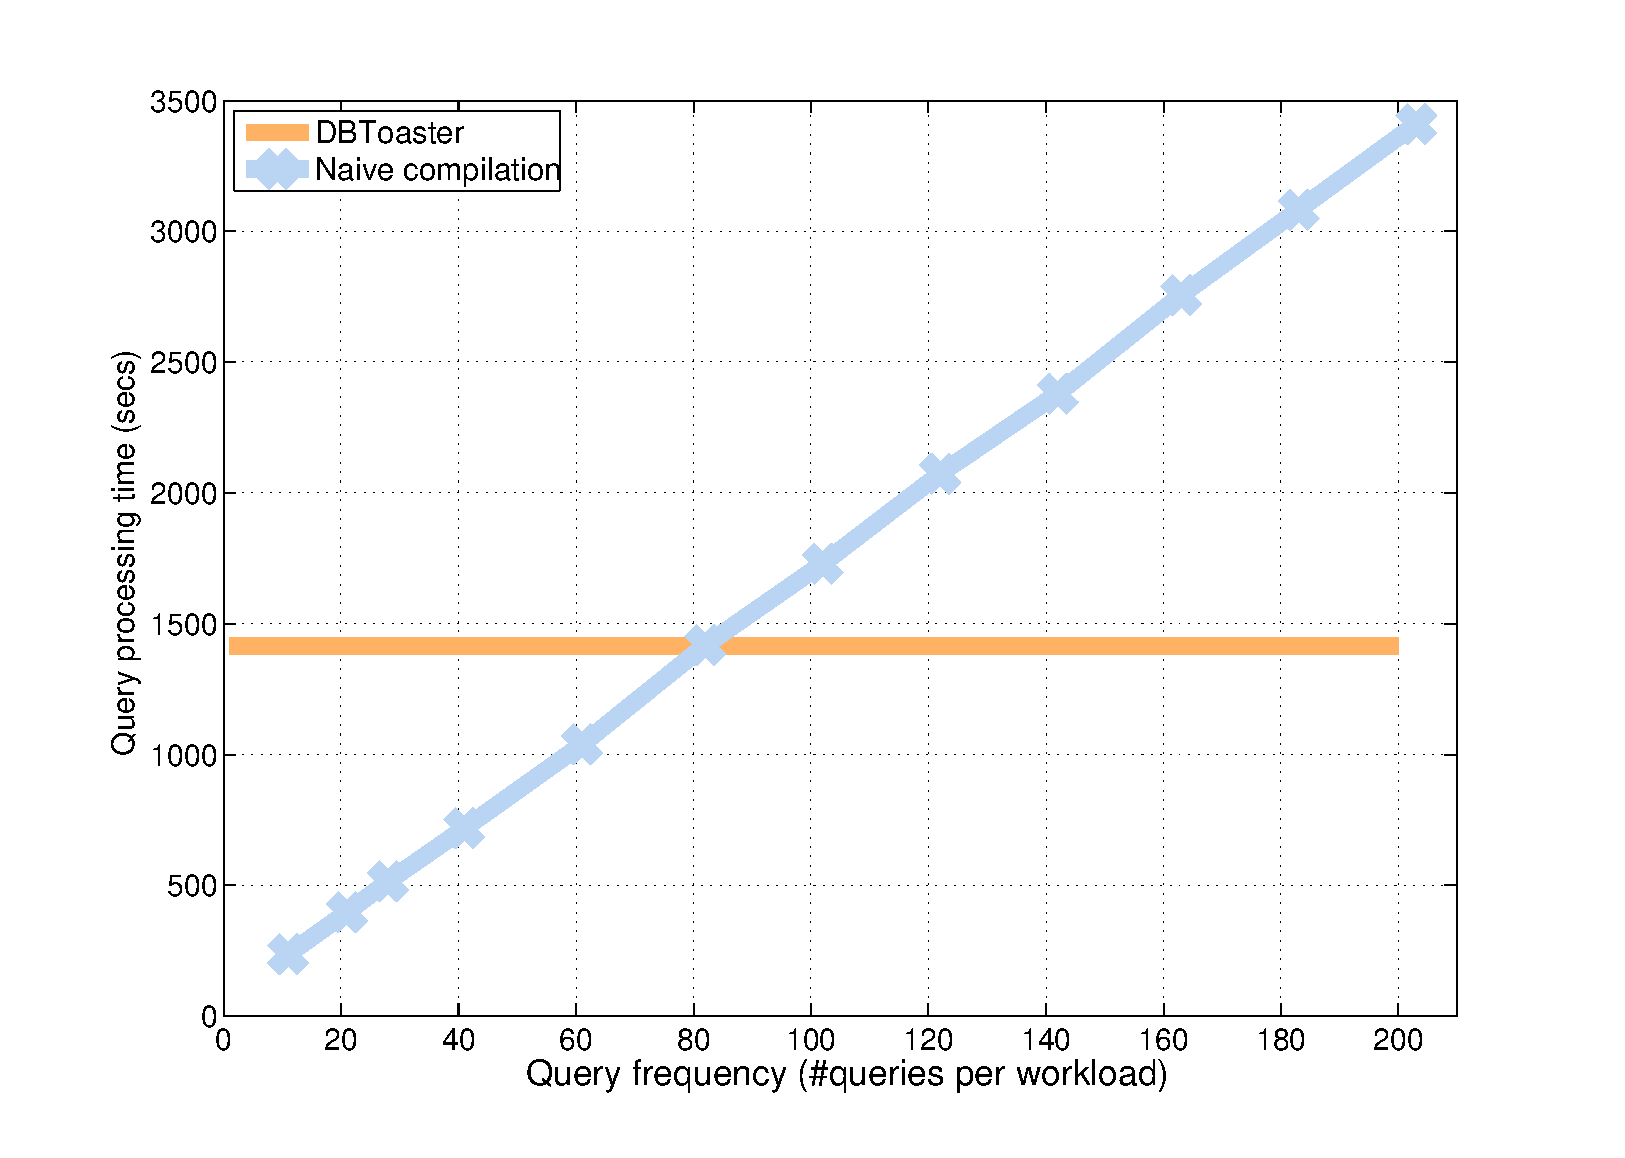
\includegraphics[scale=0.25]{../plots/vwap_query_freq_dn}
\end{center}
\caption{Query frequency limit for VWAP application, indicating the
query execution frequency beyond which DBToaster outperforms the naive query
plan compilation technique.}
\label{fig:vwap_query_freq}
\end{figure}

\begin{figure}
\begin{center}
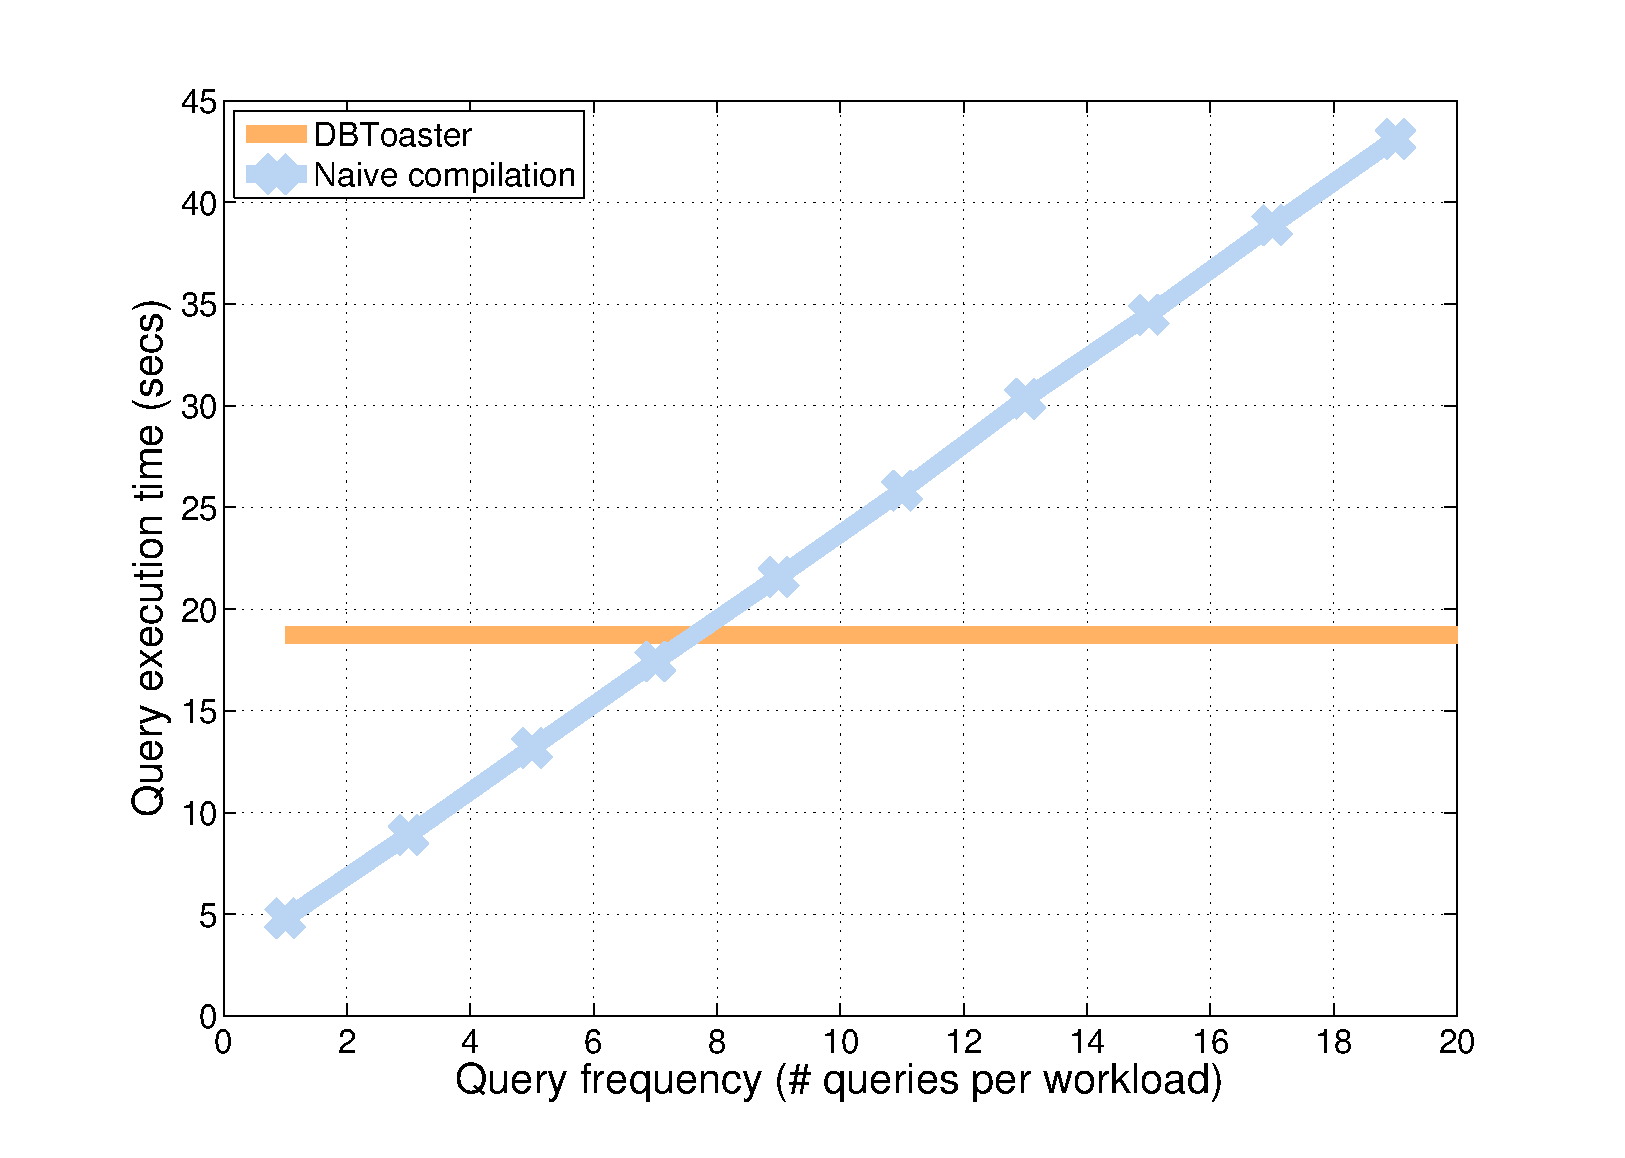
\includegraphics[scale=0.25]{../plots/ssb_query_freq_dn}
\end{center}
\caption{Query frequency limit for warehouse loading application, indicating the
query execution frequency beyond which DBToaster outperforms the naive query
plan compilation technique.}
\label{fig:ssb_query_freq}
\end{figure}

\subsection{Memory Analysis and Batch Execution}


\comment{
Dataset:

\begin{itemize}
  \item TotalView-ITCH dataset: 3 month's worth of MSFT order book messages
  taken from NASDAQ, (~2.2Gb dataset).
  \item Orderbook schema: day, time in us since beginning of day, order id,
  order type, share volume, bid/ask price
\end{itemize}

Queries:

\begin{verbatim}
select * from
  (select ax_bids.mmid, abs(
    sum(ax_bids.volume*
      (act_now.expected_price - ax_bids.price)) -
    sum(ax_asks.volume*
      (ax_asks.price - act_now.expected_price)))
    as ax_bias
  from
    (select mmid, price, volume from bids
       where mmid in axs) as ax_bids,
    (select mmid, price, volume from asks
       where mmid in axs) as ax_asks,
    (select expected_price
        from technical_indicator
        where entrance_condition)
    as act_now
  where ax_bids.mmid = ax_asks.mmid
  group by ax_bids.mmid) as sneaky_ax,
where ax_bias > 10000
\end{verbatim}

Figures:

\begin{enumerate}
  \item Takeaway experiment: end-to-end throughput comparison for a variety of
  insert/update/delete rates. Requires replay speed parameter in data loader.
  Comparison points include Postgres, naive compilation, simple version
  of \compiler, \compiler\ with lazy evaluation, \compiler\ with bulk insert
  mode at 2 or 3 different chunk sizes.

  \item Detail experiment: analyse effect of bulk loading operations compared to
  simple compiler, on a variety of queries, e.g. selectivities and keys.
  Dependent variables for plots: cache hit rates for locality analysis,
  throughput to understand pipelining effects. Is there anything lower lever we
  can do for pipelining?

  \item Detail experiment: selectivity experiment, comparing \compiler\ w/ lazy
  eval, and w/ bulk loading (separately) to next best, for a variety of
  join selectivities and keys.

  \item Detail experiment: space vs recomputation analysis, where we vary the
  maps we keep between extremes of maps from simple decomposition, to full base
  tables.

  \item Quality of compiled code, and compiler effect? e.g. speed provided with
  different -O flags?

\end{enumerate}
}
\section{Related Work}

To the best of our knowledge, there has been limited work addressing the question
of how to compile SQL queries to a low-level imperative language such as C++.
With this in mind, in this section we contrast our map algebra, query rewriting
and execution to several more extensively investigated topics, namely view
maintenance, main-memory databases as well as stream and event processing.

\textbf{View maintenance.}
View maintenance algorithms are in abundance in the database literature, with
topics ranging from efficient view maintenance algorithms given base relation
deltas~\cite{colby-sigmod:96}, which may be eagerly or lazily
applied~\cite{yan-vldb:95,zhou-vldb:07}, to the question of which views to
actually materialize and how to use such views during query
optimization~\cite{kotidis-tods:01,zhou-icde:07}. Zhou et. al~\cite{zhou-vldb:07}
describe a lazy view materialization technique, describing their computation of
deltas starting from a similar point to ours, namely that where a single tuple
has changed as part of a join tree input. However, their approach does not
generalize to the same extent as our map algebra, particularly in the case of
nested aggregations such as the VWAP query seen in this work. Palpanas et.
al.~\cite{palpanas-vldb:02} consider an extension of view maintenance algorithms
to handle non-distributive aggregates, using a selective recomputation strategy
to update only those groups affected by new tuples. More pertinent to the
main-memory database context, Roussopoulos~\cite{roussopoulos-tods:91} presents a
pointer-based (also referred to as an index) approach to implement views with
ViewCache, which incrementally maintains views using algorithms derived from
relational operations. Griffin and Libkin~\cite{griffin-sigmod:95} study the
problem of incremental view maintenance for relations with duplicates, using a
bag algebra for equational reasoning about query operators and to derive update
rules.

Our map expression algebra differs from the issue of view maintenance, in that it
computes a set of maps to support incremental maintenance of a query result,
rather than simply maintaining a single view.
\comment{
Our approach to selecting maps under a memory constraint differs from
traditional cost models to choose views to materialize, given our top-down approach to
decomposing queries with maps.}
Furthermore, given our target application of non-interactive queries and a static
query workload, we need not maintain base relations, unlike standard relational
query processors which do so to provide ad-hoc query capability at the expense of
orders of magnitude performance as seen in our experimental section. This
obviates the need for any pointer or index-based approach to track back to
original base relation tuples, unlike existing main-memory database systems. Most
critically, the notion of compiling these view maintenance algorithms is clearly
a simple and effective technique for generating query executors for unmatched
performance.

\comment{
\begin{itemize}
  \item Asymmetric increment techniques \cite{yang-icde:05}.
  \item Group-by optimizations \cite{yan-icde:94}.
\end{itemize}
\noindent \textbf{DataCubes}
\begin{itemize}
  \item Classical literature \cite{gray-icde:96,mumick-sigmod:97}.
  \item TODO: more papers if we head into cubes.
\end{itemize}
}

\noindent \textbf{Stream and event processing.}
Our work can loosely be compared to complex event and stream processing
engines~\cite{wu-sigmod:06,agrawal-sigmod:08,white-pods:07,motwani-cidr:03,abadi-vldbj:03}
due to the common goal of handling frequently changing data.
SASE+~\cite{agrawal-sigmod:08} and Cayuga~\cite{white-pods:07} are complex event
processors that focus on sequence and pattern query processing on event streams
using NFA-based approaches to process a variety of patterns including Kleene
closures and negation operators. Relational stream processing engines such as
STREAM~\cite{motwani-cidr:03} and Aurora~\cite{abadi-vldbj:03} investigate
continuous query processing architectures that are capable of evaluating
stream-equivalent versions of the standard relation algebra. From the systems
perspective, several novel techniques were developed to address the low-latency,
high-throughput needs of stream applications, including scheduling, load
shedding, and approximate query processing.

Many of these systems are simultaneously addressing the issue of efficiency and
the semantic requirements of their target applications, naturally exploiting
application properties to attain performance. In contrast, our approach is not to
reinvent the wheel in terms of data and query models -- we focus on standard
relational algebra, and an intuitive extension via snapshots and temporal logic,
and purely take on the challenge of designing query executors to best suit a
main-memory environment, arguing for an alternative to plan-based execution.

\comment{
 TODO:
contrast our work to the above -- we avoid the need for windows or punctuations
by making adopting an insert/delete/update stream model, and assuming that the
base relations always fit in memory (i.e. \#deletes/updates is proportional to
\#inserts). Stream processors still evaluate an operator-centric query plan,
hence they cannot exploit compiler optimizations on a query processing kernel
function. They also do not deal with maintaining precomputed partial results as
we do with our map decompositions. What can we say about complex event processors
and the NFAs they evaluate?


\begin{itemize}
  \item STRIP: rule-based maintenance of derived data, with finance app example \cite{adelberg-sigmod:97}
\end{itemize}
}


\noindent \textbf{Compiling high-level languages for embedded systems.}
The embedded systems community has partially studied on compiling high-level
languages into a low-level imperative target language.
Newton et. al.~\cite{newton-lctes:08} present WaveScript, a scripting language
for processing windows, or segments, of a data stream, and describe a compiler to
construct stream dataflow graphs that are capable of running on XScale CPUs.
WaveScript programs are transformed into dataflow graphs, which may in turn be
manipulated by algebraic rewrite rules, similar to a query optimizer. However,
WaveScope does not address relational queries.
Toman and Weddell~\cite{toman-dbtel:01} describe the DEMO system which compiles
SQL queries into Java or C code, implementing query plans as navigational plans
that utilize pointer access in place of scans and indexing, and supporting query
functionality over existing data structures for an embedded program. The authors
use integrity constraints in their compiler to describe the relationship between
schemas and the physical data structures used by an embedded program, and in turn
generate navigational plans and iterators, which can be used to produce C code in
a straightforward manner. DEMO has taken a theoretical approach to describe
their compilation, and does not consider systems issues nor have they released
a prototype and provided an effective tool to perform compilation.


\noindent \textbf{Main memory databases.}
Early work on main-memory databases studied how to reduce the bottleneck effect
of a variety of I/O tasks including recovery tasks such as checkpointing, as well
as logging and locking structures \cite{bohannon-vldb:98,bohannon-sigmod:99}.
There have been several recent efforts on this topic given the developments in
main memory.

Boncz et. al.~\cite{boncz-cidr:05} present the MonetDB/X100 database engine, a
high-performance column-oriented database, that leverages techniques such as
vectorized processing and loop pipelining on chunks of columns while evaluating
operators in query plans. Kallman et. al.~\cite{kallman-pvldb:08} describe
H-Store, a shared-nothing distributed main memory database to provide high
throughput processing on OLTP workloads. H-Store achieves its performance through
careful deployment of horizontally partitioning of relations, and localizing OLTP
transactions to partitions. Raman et. al.~\cite{raman-icde:08} describe Blink, a
row-oriented main memory query processor that extensively uses compression on
denormalized relations, and applies aggregates while scanning these relations as
its main query processing functionality.

These systems span a wide variety of use cases and focus at rearchitecting at a
lower-level than the our approach. For now we have looked at applying a semantic
redesign to describe queries as tuple functions, and reuse much of the work from
the compiler community to provide efficient tuple function execution. Having
applied this first phase to building our runtime, we can now proceed to the
systems level aspects of our tuple functions, for example investigating cache
performance in much greater depth, and in particular understand which of the
above techniques and optimizations can be applied in our context, as well as
leveraging approaches from both the compiler and programming languages
communities in providing compiled query executors.



\section{Conclusions}

\bibliographystyle{abbrv}
\bibliography{ref}

\end{document}